\documentclass{article}
\usepackage[utf8]{inputenc}
\usepackage[margin=1in]{geometry}
\usepackage[titletoc,title]{appendix}
\usepackage{amsmath,amsfonts,amssymb,mathtools}
\usepackage{svg}

\usepackage{graphicx,float}
\usepackage[lofdepth,lotdepth]{subfig}
\graphicspath{{./graphs/}} %location of images

\usepackage[ruled,vlined]{algorithm2e}
\usepackage{algorithmic}
\usepackage{minted} 
\usemintedstyle{borland}
\usepackage{biblatex}
\addbibresource{references.bib}

% Title content
\title{Flatten, Expand, Abolish, or Just Forget about the Curve: Predicting Covid-19 Cases in Harris County}
\author{Josh Borders, Charles Colgan, Gal Egozi, Augusto Hernandez Rubio}
\date{December 5, 2020}

\begin{document}

\maketitle

% AUGUSTO: Add the name of your model to the abstract.
% Abstract
\begin{abstract}
This paper builds three different types of statistical models to attempt to accurately predict the growth of new Covid-19 cases in Harris County. The first section presents background and introductory visualization on Covid-19 case growth in Harris County. The second section introduces the types of models used: Long-Term Short Memory, time series regression with cyclical trend, and a standard linear regression. The third section fits case counts to the models and presents results. The fourth section concludes the paper by discussing the advantages and disadvantages of the respective models.
\end{abstract}

% Intro and Viz
\section{Jiggles, Wiggles, and Waves: An Introduction}
For all the damage Covid-19 has wreaked on the world, it has brought with it a renewed interest in statistical modeling. At the beginning of the pandemic, a different model with different methodologies entered the limelight seemingly every day, with predictions on case counts, economic consequences, and fatalities growing increasingly dire. While most of the model-building was left to seasoned statisticians and epidemiologists, laymen could even get in on the action, tracking case growth with the help of popular websites.\\\\
The prevalence of models and interpretations thereof has led to an interesting question: which model is most accurate at modeling the spread of Covid-19? Should public health authorities use machine learning models, or will traditional regression models do?\\\\
This paper attempts to answer this question in an admittedly narrow way, by examining the performance of four different models when predicting new Covid-19 case growth in Harris County, Texas. Our data set is titled "New Cases over Time by County" from Texas's Health and Human Services website.\footnote{https://dshs.texas.gov/coronavirus/AdditionalData.aspx} We focus on Harris County, specifically the observations from March 4, 2020 - when data was first recorded - to November 30, 2020: a period of 269 days.\\\\
The new case counts over the 269-day period are displayed in red in Figure \ref{new_cases}. It shows a wave-like pattern, as there was a brief surge of cases right after April, a more sustained wave over the summer, trending downward in early autumn, and then the most recent spike toward the end of November. In blue, a simple linear regression of case count on time is presented. While the general positive trend is correct, it basically slices the actual case numbers in two, undershooting the values for half the graph, and overestimating them for the other half.
\begin{figure}[H]
    \centering
    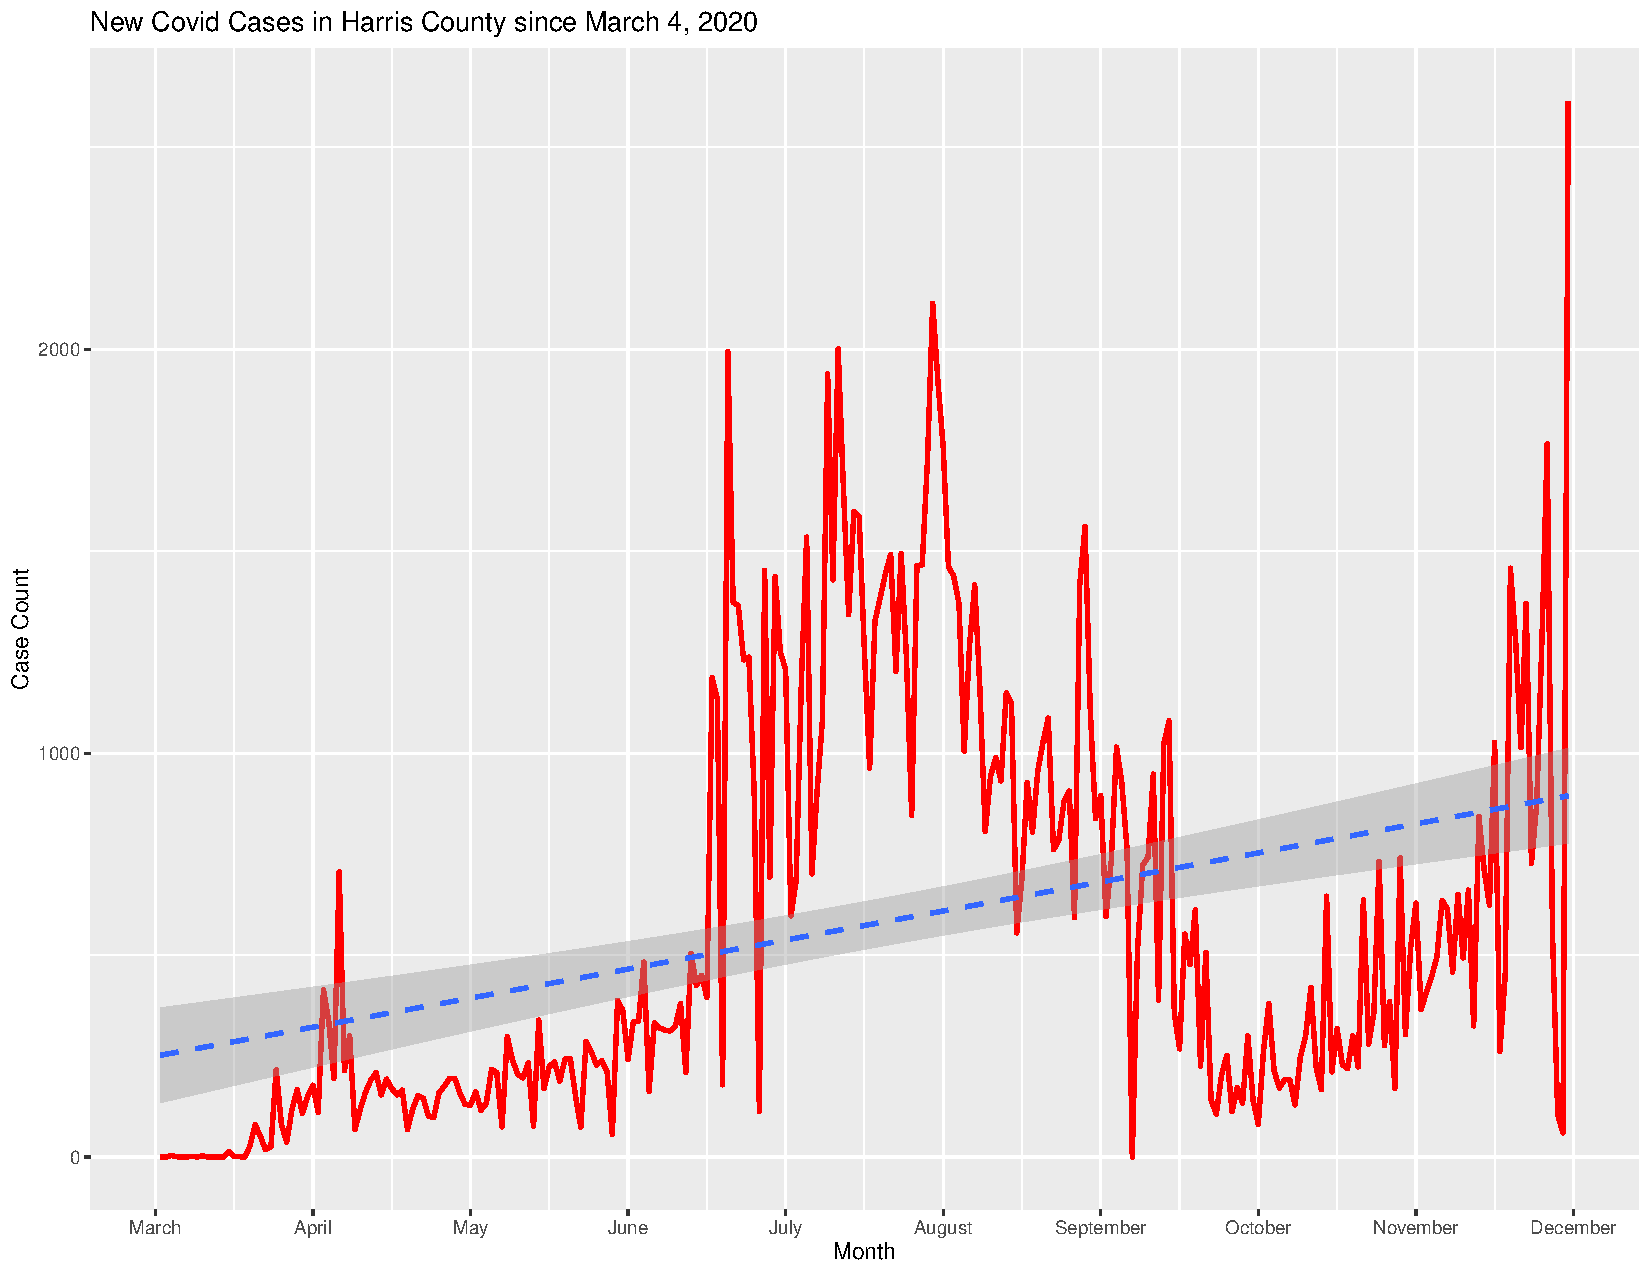
\includegraphics[width=12cm,height=7cm]{graphs/new_cases.pdf}
    \caption{Harris County New Covid-19 Cases over Time}
    \label{new_cases}
\end{figure}
In other words, a simple linear regression will not be appropriate for this analysis. Therefore, we will introduce different models to try to predict case counts in Harris County.

%  Model Specs
\section{Introduce Me to Your Model Friend: Specifying the Models}
We now introduce the three different model types used to predict the case counts: Long Short-Term Memory, time-series regression with cyclical trend, and a standard linear regression model. Each subsection is devoted to a specific model type.

\subsection{Long Short-Term Memory - by Gal Egozi}
There are two ways to do time series prediction, one is to design a function $f(t)$ that predicts the COVID cases as a function of time. Another model is to predict the COVID cases based on the previous days, so that the number of cases on any particular day is predicted by the number of cases in previous days. A function of this form would be like $f(t) = g(t-1,t-2)$, where $g$ is used to predict $f(t)$ based on previous values of $t$. Because of the cyclical nature of COVID 19 and the fact that the CDC recommends a 14 day quarantine for exposure, the previous 14 days are used to predict the next day. The current architecture is shown below, along with some code required to get the model running. The training runs for 1000 epochs.
\begin{minted}[linenos]{python}
from tensorflow.keras.models import Sequential
from tensorflow.keras.layers import LSTM, Dense, Bidirectional
from tensorflow.keras.optimizers import Nadam
model = Sequential([
    Bidirectional(LSTM(2000)),
    Dense(100, activation='relu'),
    Dense(100, activation='relu'),
    Dense(1)
])
opt = Nadam()
model.compile(loss='mean_squared_error', optimizer=opt)
history = model.fit(training, epochs=1000)
\end{minted}
This model requires more code; however, this snippet shows the key part, the architecture of the model. While it would be difficult to express the model as a mathematical function, the above code shows the form of the function, in the same way that $y=mx+b$ expresses the form of a linear regression. The equation is much more complicated and has many more variables, so this segment of code replaces the explicit equation.

\subsection{Time Series with Cyclical Trend}
The cyclical trend model attempts to predict the new case counts by incorporating sine and cosine curves into a typical time-series regression, where time has some effect on the dependent variable. The predicted regression equation is,\begin{equation}
    Cases_i = \hat{\beta_0} + \hat{\beta_1}Day_i + \hat{\beta_2}Cases_{i-7} + \hat{\beta_3}Cases_{i-14} + \hat{\beta_4}sin(\frac{2\pi}{14}Day_i) + \hat{\beta_5}cos(\frac{2\pi}{14}Day_i) + \hat{\epsilon}
\end{equation}
where \textit{Cases$_i$} is the number of new cases on \textit{Day$_i$}, with \textit{Day$_i$} being the number of days since Texas's statewide Covid-19 database was established on March 4, 2020; March 4th is considered \textit{Day$_1$}. \textit{Cases$_{i-7}$} is the case count seven days before the \textit{i}th day, and a similar interpretation is given to \textit{Cases$_{i-14}$}. The model looks back in time by both one and two weeks, \textit{Cases$_{i-7}$} and \textit{Cases$_{i-14}$}, respectively, for two reasons. The first is domain-specific. Since the virus is expected to have a two-week incubation period, it's good old-fashioned common sense to include variables looking back at the previous two weeks of observations. The choice of one week back and two weeks back feeds into the second justification for their inclusion into the model: auto-correlation. Figure \ref{autocorr} displays the average auto-correlation coefficients between the present observation and the \textit{x} previous. For example, the present observation and the observation from five days prior are correlated at about 0.75. There are noticeable spikes in correlation at \textit{Day$_{i-7}$} and \textit{Day$_{i-14}$}, which aligns with consensus knowledge of the virus. Therefore, the case counts from these days, \textit{Day$_{i-7}$} and \textit{Day$_{i-14}$}, were included in the model. Lastly, the sine and cosine terms are included to capture cyclical fluctuations in the case count. Figure \ref{new_cases} shows a possible harmonic pattern in the case counts. The period of the functions were set, after trial-and-error, at two weeks, once again aligning with domain knowledge of the virus.\\\\


\begin{figure}[h]
    \centering
    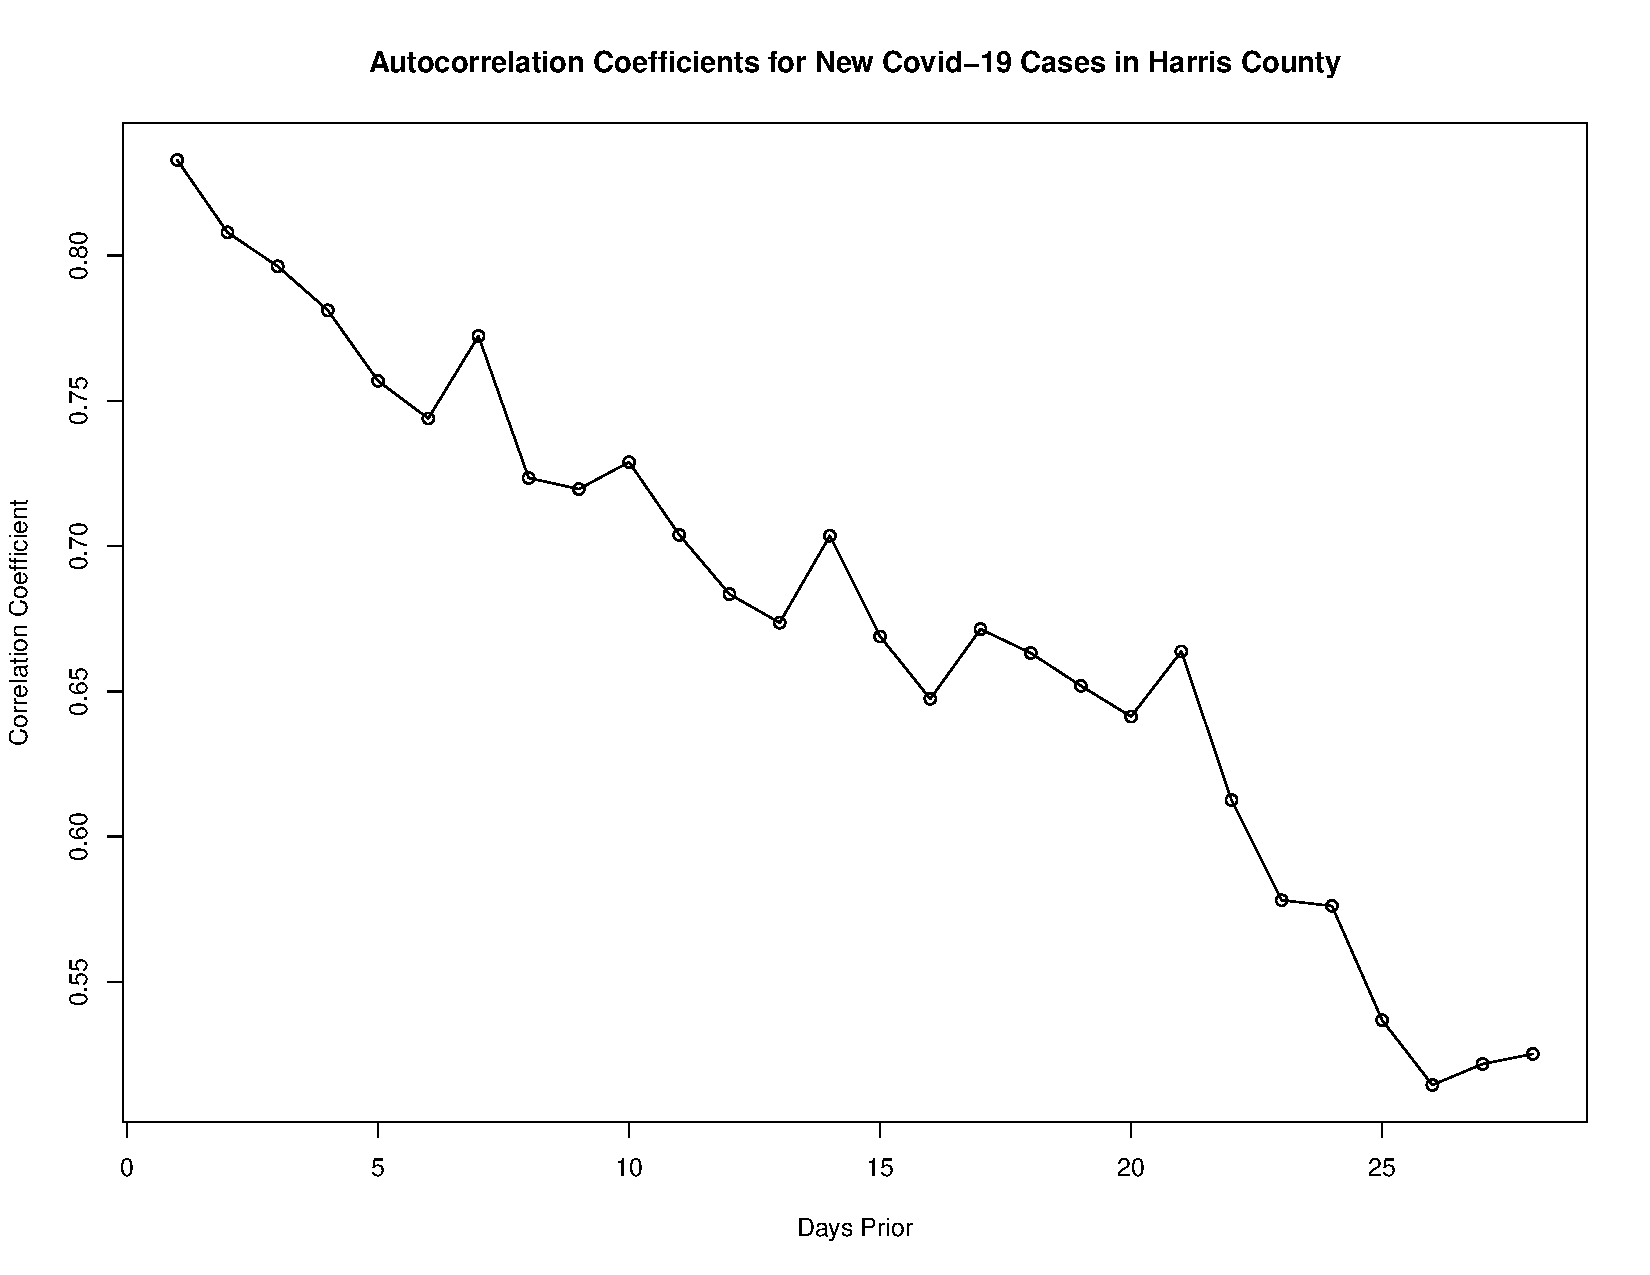
\includegraphics[width=12cm,height=8cm]{graphs/ac_coeff.pdf}
    \caption{Auto-Correlation Coefficients between Observations}
    \label{autocorr}
\end{figure}

\subsection{Standard Linear Regression}
As a point of comparison, we have also included a model for a standard linear regression. Linear Regression is the process of determining a linear relationship between result and any number of predictors. This is accomplished by assuming a linear predictor function, $Y=\beta_0+\sum_{i=1}^n\beta_iX_i+\epsilon_i$, where $Y$ is the result we seek to predict and $X$ is the value of the predictors we seek to use, whose effect on the result is given by $\beta$. $\epsilon$ is the difference between the results of our model and the known results, called the residuals. In order to do this, we estimate the the values of $\beta$ from the data. We then form a predictor function and generate a predicted result using the values of our predictors. Comparing our predicted results to our recorded gives us our residuals. The residuals are extremely useful, as they allow us to asses how well our model is able to match our observed data.\\\\
One approach to this is to create what are known as residual plots and Quantile-Quantile (QQ) plots. A residual plot consists of the residuals of a linear regression plotted against the values of the the predictors. This gives a graph where the plotted points appear on either side of the zero line. Depending on the displacement of the plotted points, the adequacy of using a model of the form the residuals originated from can be determined. The more random the points are, the more adequate the model. If instead there is clear and non-random behavior, the model is likely inadequate. A QQ plot consists of the residuals of a linear regression plotted against a theoretical normal distribution. This gives a graph where the points plot a line through the origin. The closer the points are to a line of slope one, the more normal the residuals are and thus the data is. If instead the point deviate greatly from a straight line, then the residuals are non-normal, as is the data. One can also directly compare a plot of the recorded results to the predicted ones. Doing so allows one to look for differences that might not be visible from the residuals alone.

\section{It May Be a Tight Squeeze: Fitting the Models}

\subsection{LTSM - by Gal Egozi}
The LSTM uses the previous 14 days to predict the next day. Unlike RNNs, it retains a longer history. Because the LSTM uses the previous days to predict the next, it can get very high accuracy, but takes a considerable amount of time to fit and perform hyperparameter tuning. Figure \ref{LSTM_predictions} shows the LSTM predictions and the actual case counts per day. It is more accurate in the training portion (the first 70\%), but it still gets the main trends of COVID 19 for the remaining days. It clearly struggled predicting the high variability in daily cases near the end of the dataset (the end of November). The LSTM may not be able to predict the periods of high variability that it has not seen, but it is able to model the trend of the dataset.
\begin{figure}[h]
    \centering
    \includesvg[width=12cm,height=8cm]{graphs/gal-predictions}
    \caption{The LSTM predictions (blue) with the actual case counts (orange)}
    \label{LSTM_predictions}
\end{figure}

\subsection{Time Series with Cyclical Trend}
This model trained on the first two-hundred days of the pandemic, leaving the latter sixty-nine observations for validation. This is roughly a 75-25 split, standard for time-series analysis. The estimated regression model is, \begin{equation}
    \hat{Cases_i} = -165.06 + 7.33Day_i + 0.30Cases_{i-7} + 0.46Cases_{i-14} + 22.54sin(\frac{2\pi}{14}Day_i) + 37.58cos(\frac{2\pi}{14}Day_i)
\end{equation}
where the coefficients can be interpreted as follows. Holding all other variables constant, every additional day into the outbreak is expected to yield 7.33 additional Covid-19 cases. The coefficients on the back-shift terms are both positive, indicating that 30\% of the case count from seven days ago is expected to be added on to the \texit{i}'th day's cases, likewise 46\% of the cases from fourteen days ago. The harmonic terms are more difficult to interpret, but they attempt to approximate cyclical variation in the cases over a two-week period.\\\\
The R output for the estimated regression is in Figure \ref{cyc_output}. The model explains approximately 63.7\% of the variance in the number of cases. Every variable is significant at the 1\% level, except for the sine and cosine terms, which are not significant at any reasonable level. A reduced model without the sine and cosine terms performs just as well as the full model. Trials with different periods for the sine and cosine terms yield similar results.\\\\
Though all metrics suggest dropping the sine and cosine terms is wise, sometimes it is instructive to look at the residuals. Figure \ref{cyc_resid} shows two plots: one a qq plot of the residuals, the other a plot of the residuals versus the fitted values. While the qq plot is a bit wavy, it does follow the normal line relatively well. Additionally, there is not much of a pattern when plotting the residuals against the fitted values. These indicate a relatively-well fit regression model, even when including the "insignificant" harmonic terms. Though they may not have small p-values, they are still appropriate to include in this, a cyclical trend model.\\\\
The estimated regression function is now used to predict observations it had not previously seen, the 69 points from the training set. A plot of the actual vs. predicted values for the training set is shown in Figure \ref{cyc_train}, with a line of y=x provided for scale. Points closer to the line are more accurate in their prediction. The model consistently over-estimates the number of new Covid-19 cases Harris County experienced from late September to the end of November. More rigorous metrics of the model's performance on the test set, including AIC and MSE, are provided in Section 3.4.

\begin{figure}[h]
    \centering
    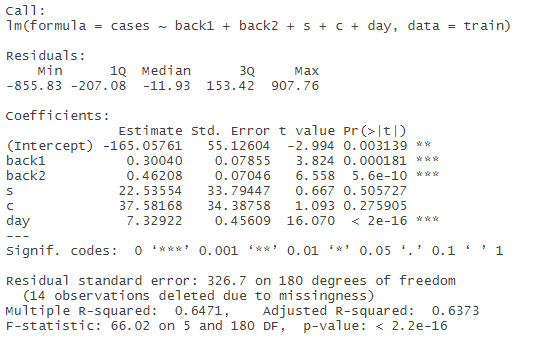
\includegraphics[width=9cm,height=5cm]{graphs/cyc_train_output.png}
    \caption{R Output for Cyclical Trend Regression}
    \label{cyc_output}
\end{figure}

\begin{figure}[h]
    \centering
    \subfloat[Residuals vs Fitted Values]{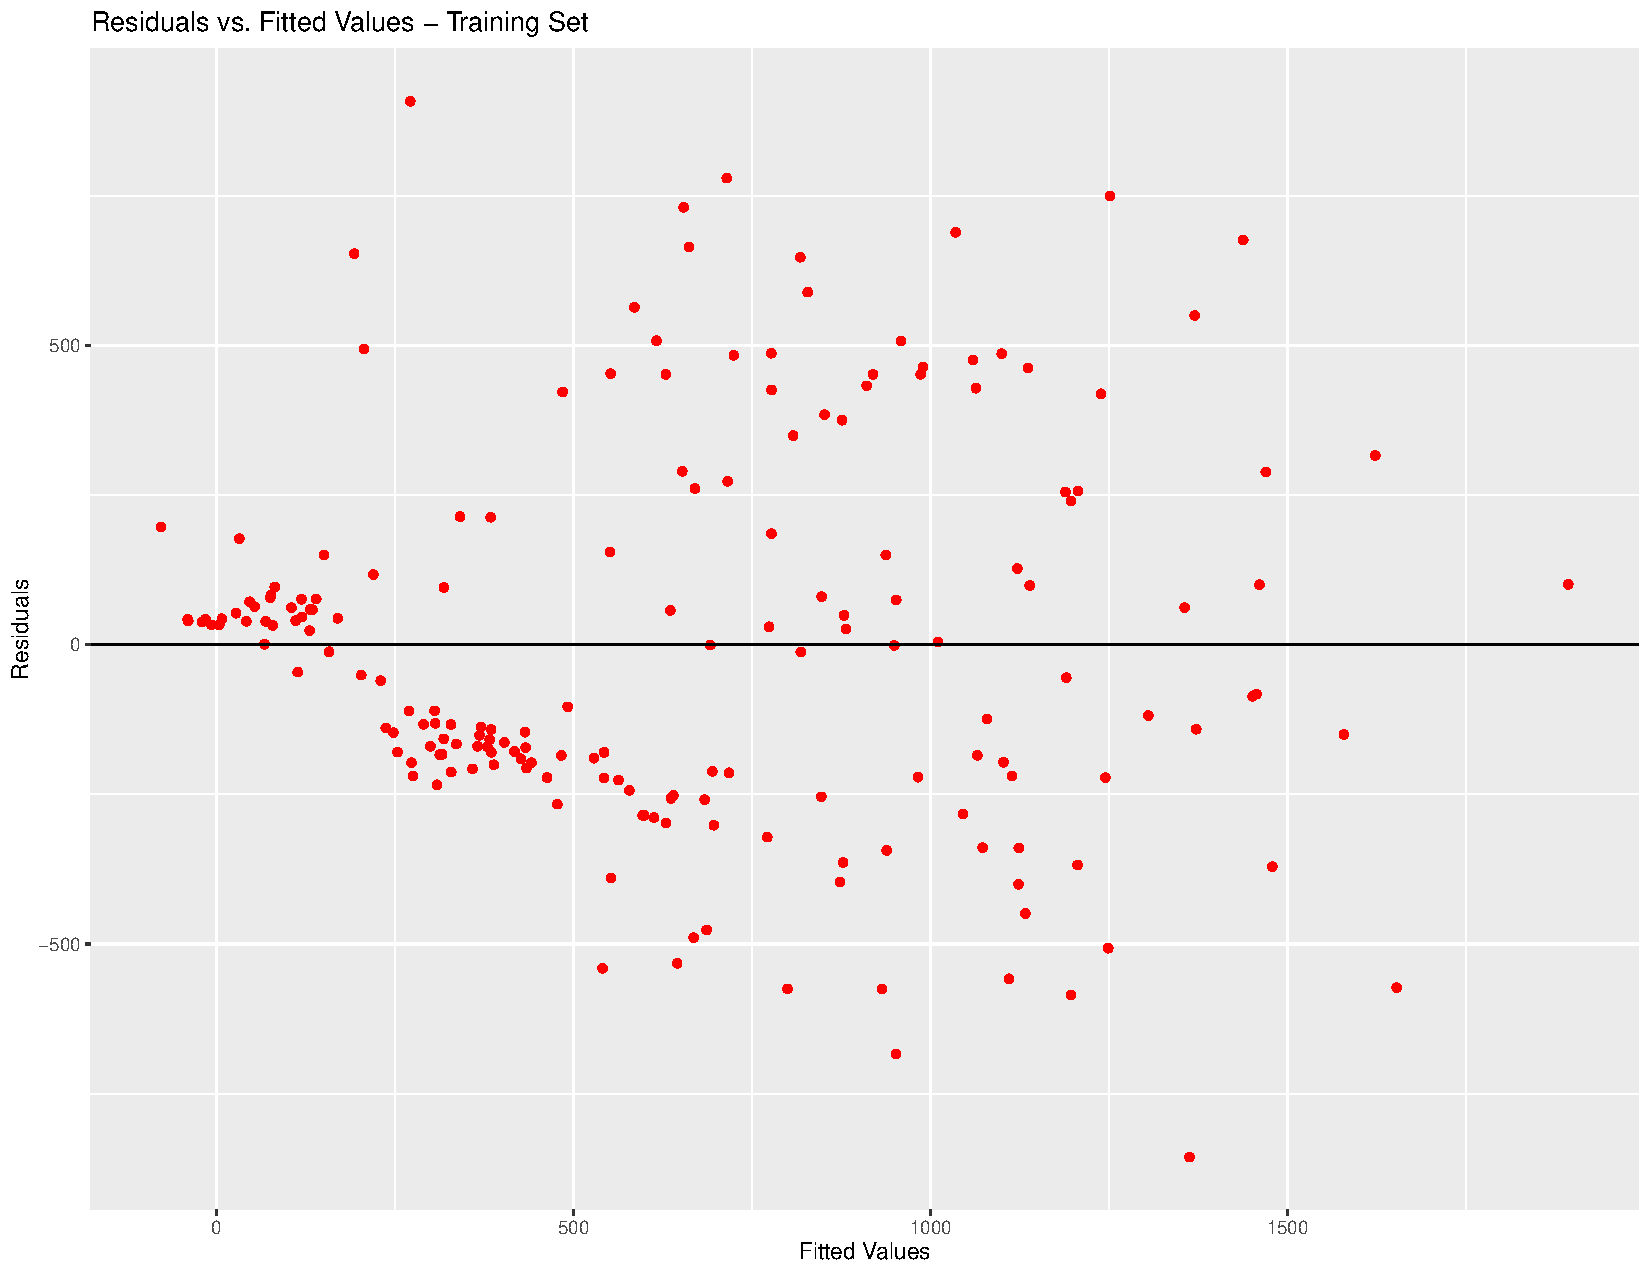
\includegraphics[width=9cm,height=6cm]{graphs/cyc_resid_fit.pdf}} 
    \subfloat[QQ of Residuals]{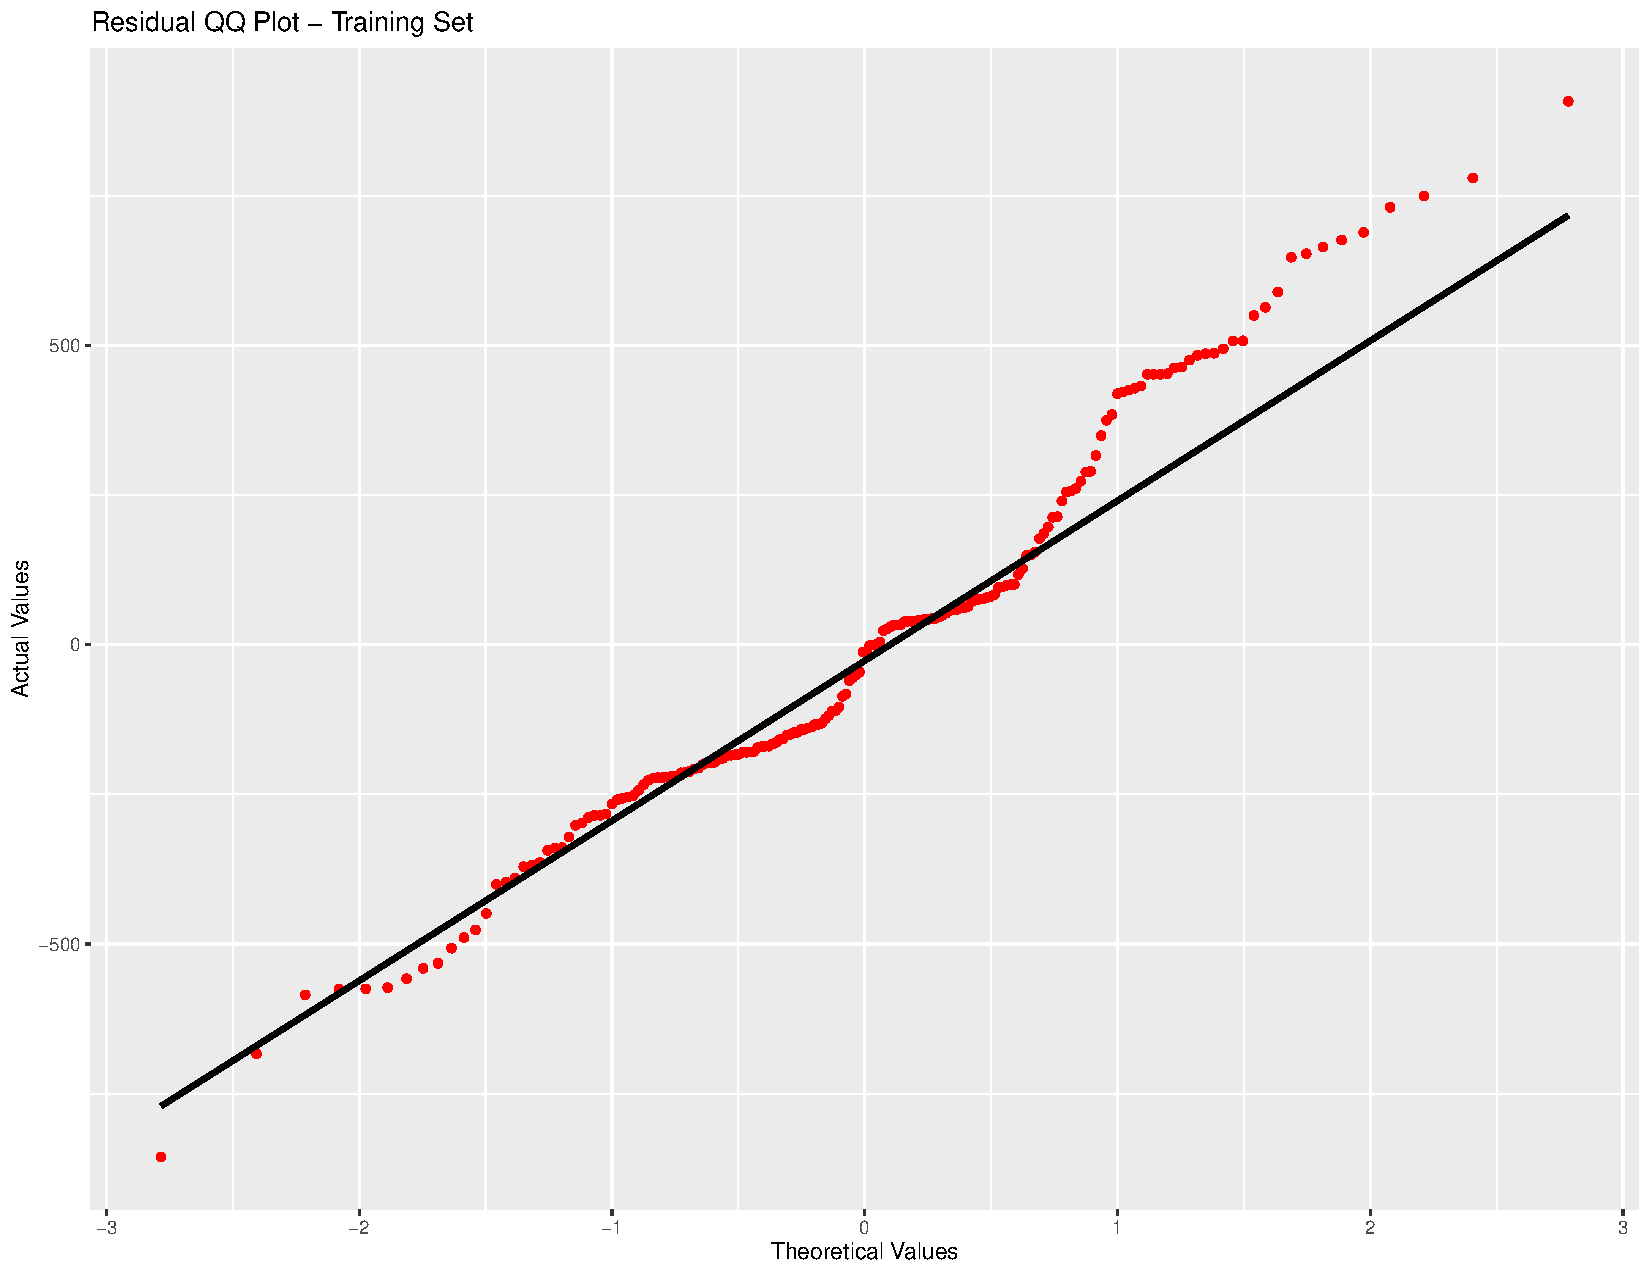
\includegraphics[width=9cm,height=6cm]{graphs/cyc_qq.pdf}} 
    \caption{Residual Plots - Training Set}
    \label{cyc_resid}
\end{figure}

\begin{figure}[h]
    \centering
    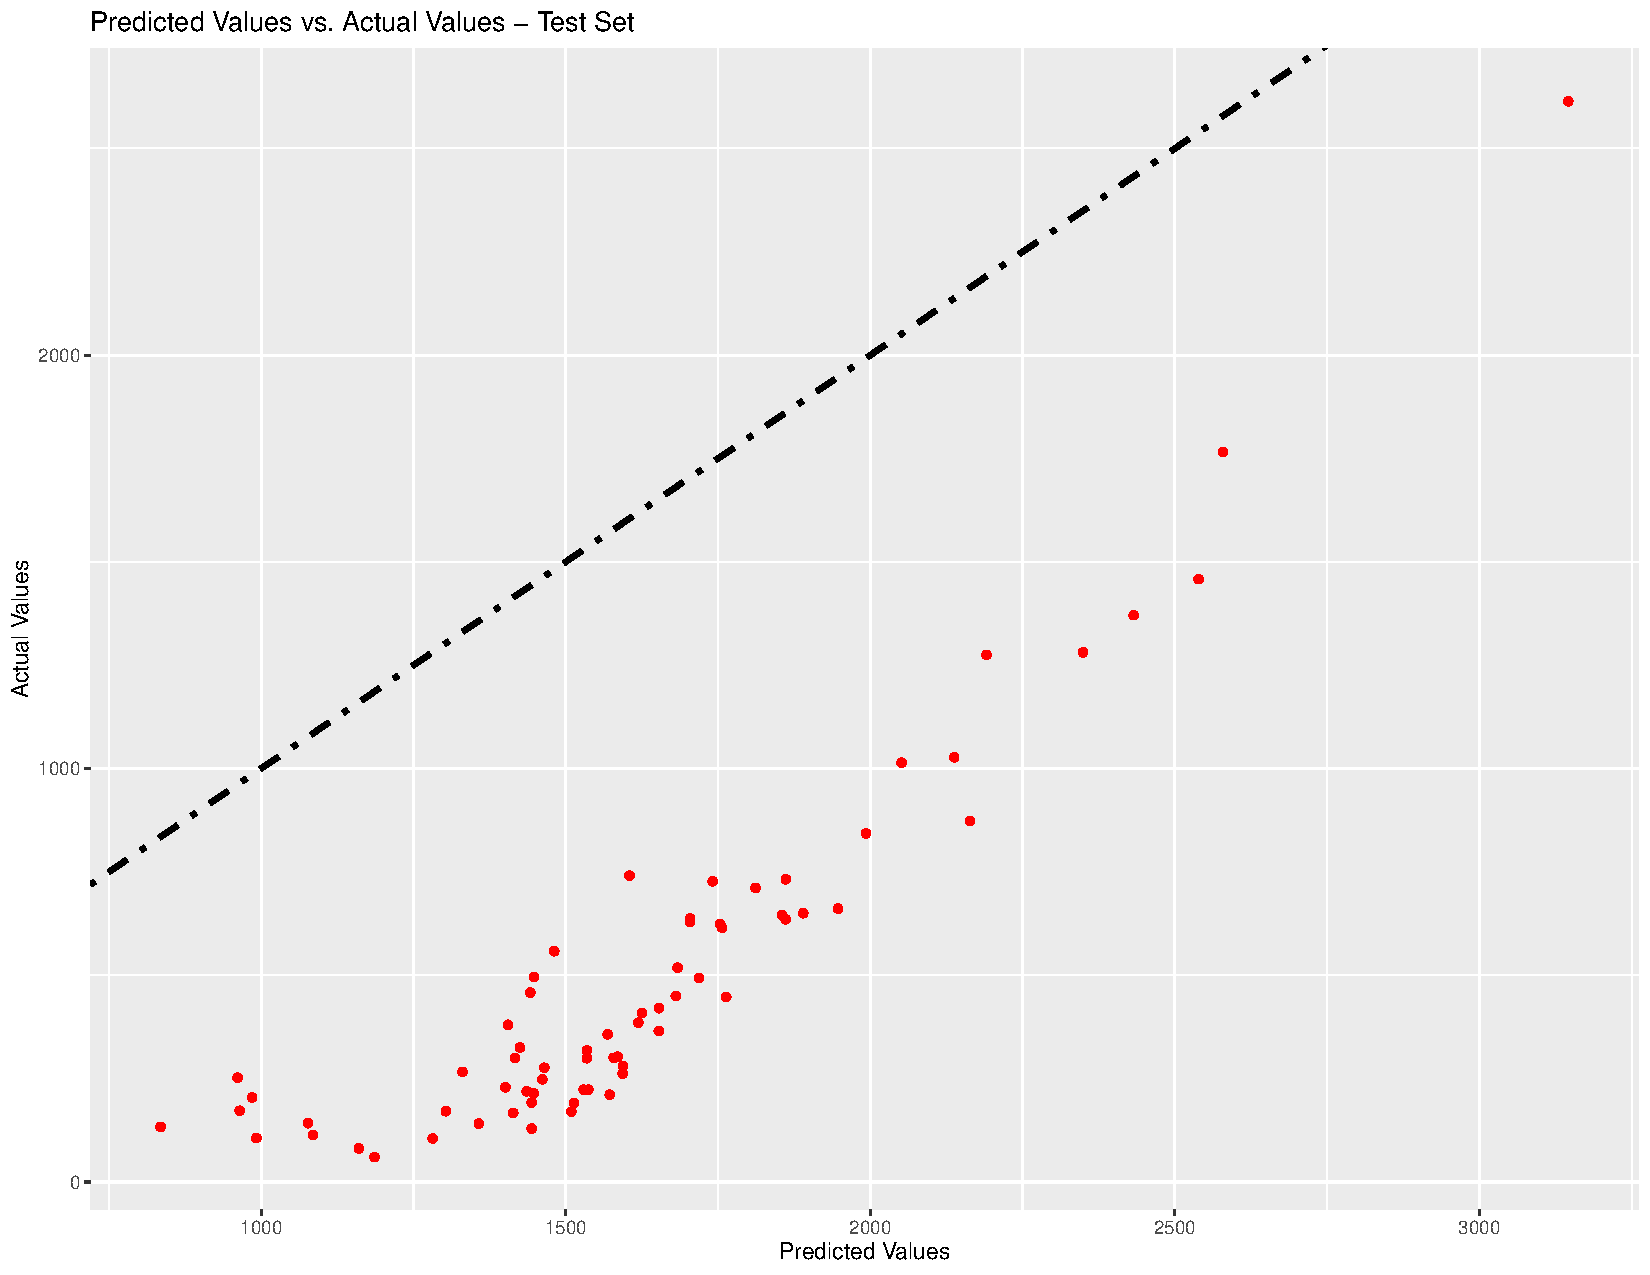
\includegraphics[width=8cm]{graphs/cyc_test.pdf}
    \caption{Actual Values vs. Predicted Values - Test Set}
    \label{cyc_train}
\end{figure}


\subsection{Standard Linear Regression}
For our model we used the days since case recording started to predict the number of reported Covid-19 cases in Harris county, Texas. By our stated model, we used $Y_{cases}=\beta_0+\beta_1X_{day}$ as our linear prediction function. After preforming linear regression we obtained values for $\beta_0$ and $\beta_1$ of -38133.59 and 806.26, respectively. While our $R^2$ (a measure of how much variance in the result is due to the predictors) is 0.9435, indicating a high amount of explained variance, as can be seen in Figure \ref{fig:Full_fit}, this model does not fit our data well.\\\\
\begin{figure}[H]
    \centering
    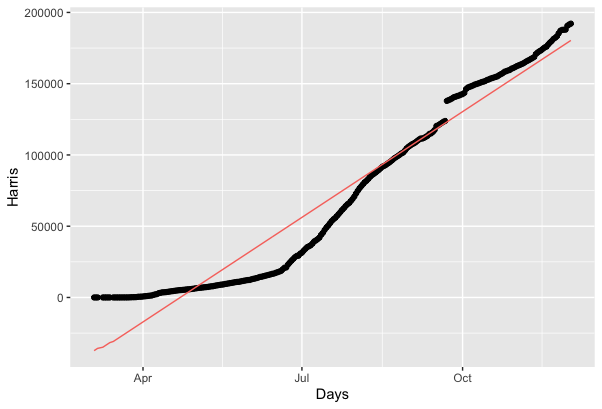
\includegraphics[width=8cm,height=6cm]{Full_fit.png}
    \caption{Fit versus Data. Fit in red}
    \label{fig:Full_fit}
\end{figure}
Looking at the residual and QQ plots of our data (Figure \ref{fig:QQ_Res}), we see that our assumption that the model does not fit well is supported. The residual plots display a large amount of non-randomness, thus indicating that our model is very iinadequate. The QQ plot, while close to normal, does contain several instances where we diverge from normality. This indicates, while our data is for the most part normal, there are significant deviations from normality.\\\\
\begin{figure}[H]
\centering
\subfloat[Residual Plot]{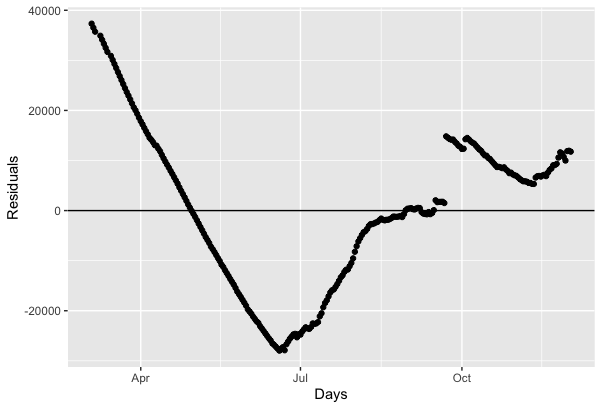
\includegraphics[width=7cm,height=5cm]{Full_Res.png}}
\subfloat[QQ plot]{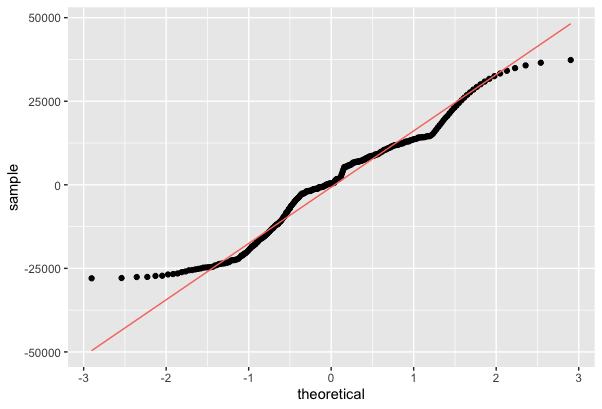
\includegraphics[width=7cm,height=5cm]{Full_QQ.png}}
\caption{Residual plot and QQ plot}
\label{fig:QQ_Res}
\end{figure}
In order to combat this, We redesign are our model. From Figure  \ref{fig:Full_fit}, we can see that certain sections of the data are approximately linear, though they have different forms. The most general of these are approximately from the beginning of case recording in March to July, from July to October, and then from October to the start of December. In order to capture this feature of the data, we compute three separate linear regression, one on each of these segments. The comparison of these fits to the is shown in Figure \ref{fig:Part_fit}.\\\\
\begin{figure}[H]
    \centering
    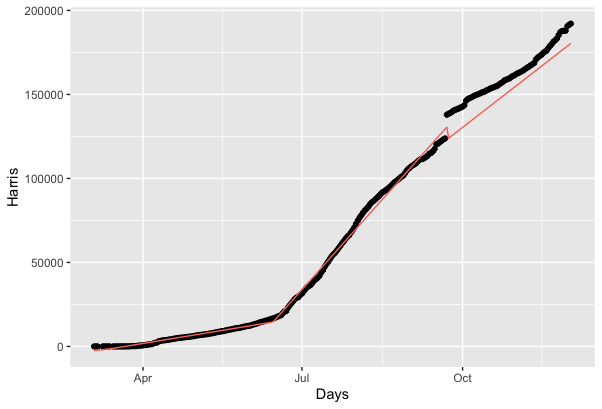
\includegraphics[width=8cm,height=6cm]{Part_fit.png}
    \caption{Fit versus Data by parts. Fit in Red}
    \label{fig:Part_fit}
\end{figure}
From the figure, we can see that our assumption that the segments of the data were approximately linear was good. Our values for $\beta_0$ and $\beta_1$ for each segment are, respectively; -2681.035 and 171.543 for March-July, -102710.05 and 1166.62 for July-October, and -8580.89 and 722.46 for October-December. Our values of $R^2$ for each segment are 0.9682, 0.9923, and 0.977. These values imply that we have captured the vast majority of the variance with our model. However, we need to take into account the information provided by the residual and Qq plots, as seen in Figure \ref{fig:Parts_Res} and \ref{fig:Part_QQ}.\\\\
\begin{figure}[h]
\centering
\subfloat[March-July]{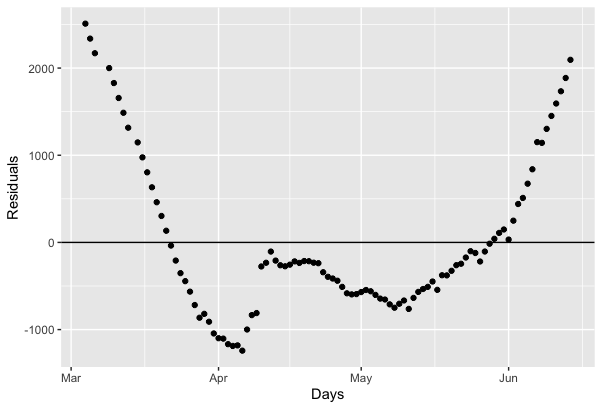
\includegraphics[width=5cm,height=4cm]{Res_P1.png}}
\subfloat[July-October]{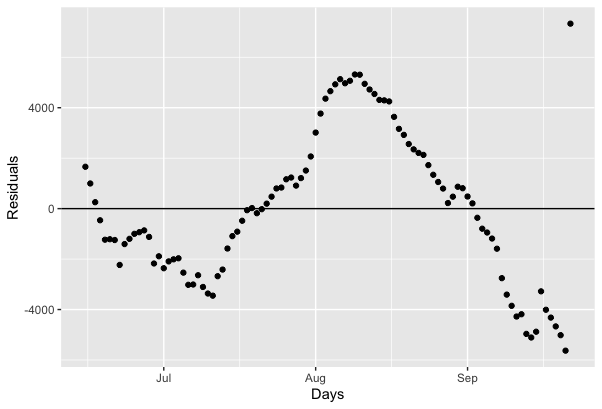
\includegraphics[width=5cm,height=4cm]{Res_P2.png}}
\subfloat[October-December]{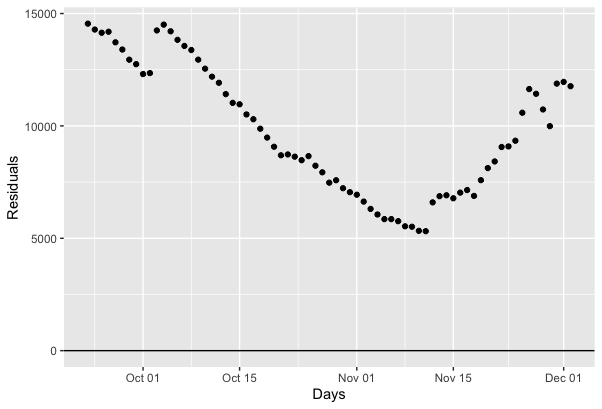
\includegraphics[width=5cm,height=4cm]{Res_P3.png}}
\caption{Plot of residuals for each group of days}
\label{fig:Parts_Res}
\end{figure}
\begin{figure}[H]
\centering
\subfloat[March-July]{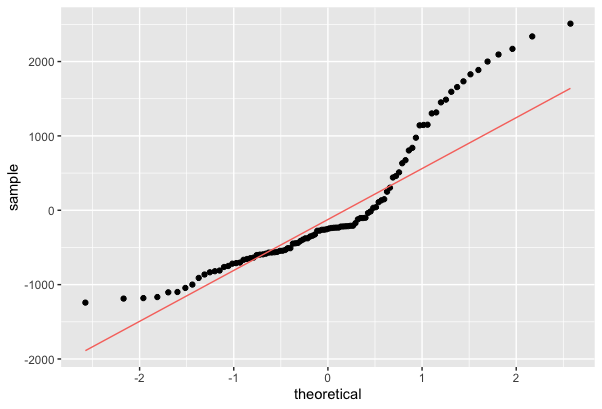
\includegraphics[width=5cm,height=4cm]{QQ_P1.png}}
\subfloat[July-October]{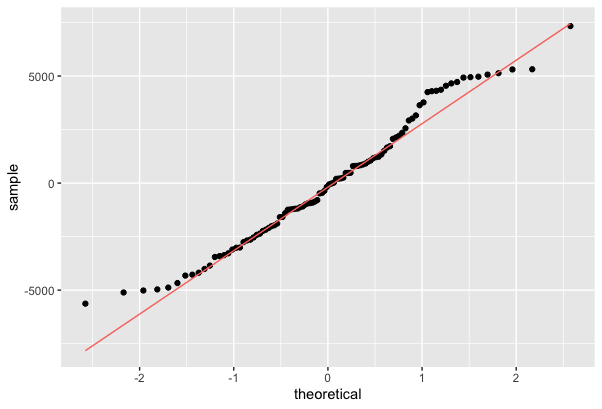
\includegraphics[width=5cm,height=4cm]{QQ_P2.png}}
\subfloat[October-Decmeber]{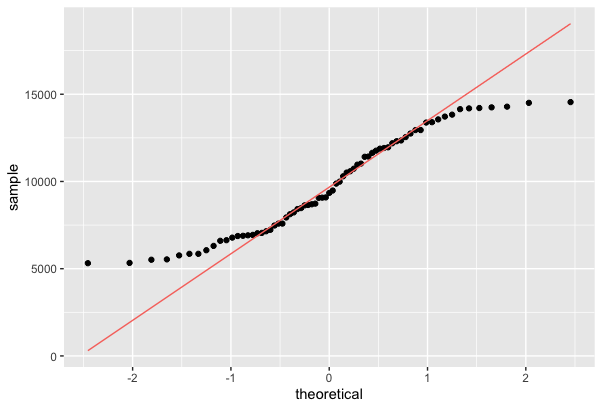
\includegraphics[width=5cm,height=4cm]{QQ_P3.png}}
\caption{QQ plot for each group of days}
\label{fig:Part_QQ}
\end{figure}
From our residual plots we can see that our use of linear models is still inadequate. While we have an improvement in randomness over regression on the data as a whole, we still have clear trends. Of note is the segment of October to December, where the all residuals are positive. By comparison with Figure \ref{fig:Part_fit}, we can see that this signals an under-fit. This likely means that there is an additional factor influencing the number of cases, besides the number of days.

Given that linear regression has its its limitations when modeling COVID-19 cases, an alternative implementation is proposed. This alternative approach is since individuals test positive days after being exposed to the virus. In this approach we are set to use active cases reported for all Texas counties, cases from date selected based on incubation period. According to the Center for Disease Control and Prevention, the 50\% of COVID-19 infections had an incubation period of 4-5 days. Given that the distribution of the incubation period is at least 5 days, we can assume that cases for a given date could have a 50\% probability to originate from a date 5 days prior to the positive test. 

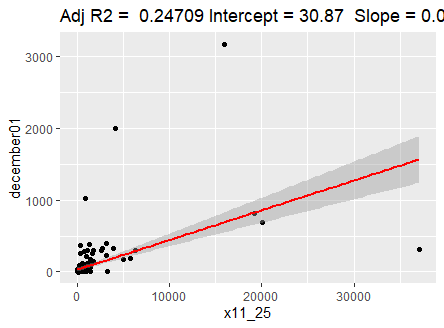
\includegraphics{Rplot01.png}
\caption{Figure 12. Linear Model for New Cases on 12-01 in relation to active on cases on 11-25}

From the linear model on figure 12 we can see that active cases 5 days before reported new infections do not seem to relate linearly to those new infections. Although the slop is not 0, the variation increases drastically as x and y get large. 

\subsection{Compiled Results}
We aggregate our respective goodness-of-fit statistics for easy comparison across different model types, displayed in Table \ref{model_stats}. R$^2$ is the proportion of variance across the dependent variable explained by the model. For an LSTM model, R$^2$ is not applicable, so none is supplied. Root mean squared error (RMSE) is defined as $RMSE = \sqrt{\frac{\sum_{i=1}^n(x_i - \hat{x_i})^2}{n}}$, where $x_i$ is the actual observation, $\hat{x_i}$ is the predicted observation, and n is the total number of observations. Mean Absolute Error (MAE) is defined similarly, with $MAE = \frac{\sum_{i=1}^n|\epsilon_i|}{n}$, where $e_i$ is the difference between the actual and predicted value.

\begin{table}[H]
    \centering
    \begin{tabular}{c|ccc}
         &R$^2$&RMSE&MAE  \\\hline
         LTSM & N/A & 243 & 117\\
         Cyclical Trend&0.844&1136&1122\\
         Standard Regression&0.9435&15435&12493
    \end{tabular}
    \caption{Model Performance on Test Set}
    \label{model_stats}
\end{table}



\section{When Curves Become Lines: Discussion and Conclusion}
Predicting Covid-19 is obviously a complicated problem.There are many confounding variables to the analysis, including the variance of government regulations, the prevalence of mass gathering events, and the fickleness of human behavior. The error term, in other words, is especially pronounced. Other reason is that positive cases don't necessarily offer information about the population. Despite the nature of the available observations (cases), we can produce models that allow us to study the current state of the virus spread. Non linear regression can be of great use when it comes to understanding fluctuations on case counts. It can also be useful to predict surges. Simple linear regression can be used for short period trends of the virus spread.  \\\\
The LSTM gives the best performance by far, but it takes the most amount of time to make a good model. The number of layers and the type of layers must be tuned perfectly. It is critical to tune the model because it can fail in many ways.\\\\
Though it explains 84\% of the variance in the test data, the cyclical trend model is hamstrung by its consistent overestimation of case counts on the test data. The overestimation is consistent in magnitude, which is encouraging, but the magnitude is large. While the model typically predicts in the right direction - higher case counts prompt even higher predicted case counts - the baseline / intercept is nevertheless off. It is possible a model like this could be useful to predict the changes in case values (i.e., whether there will be more or fewer cases x days from now), but it should not be relied upon to predict the actual values.\\\\
While each model has its advantages, the LSTM is the best of the three we examined. 

The LTSM produced predictions that resembles the data the closest. While LTSM offers better prediction than other models, it is also computationally heavy. The LSTM does the best, with the Cyclical Model next, and finally the Linear regression. In terms of RMSE and MAE, there are significant variations between the three models, where the LSTM performs between 5-10x better than the Cyclical model and approximately 100x better than the linear regression. The standard regression has the largest R$^2$, but that is likely a coincidence because of the data. It is clear that the cyclical and LSTM are able to predict the daily cases much better. The LSTM, with its large amount of parameters, can be tuned to minimize the RMSE and the MAE much further than any other model. A linear regression is simple to train, but has too few variables to accurately model this chaotic data. Our models could be improved by taking into account the average period a person remains infectious, and the effective reproduction rate. 

\end{document}
